\section{Laufzeitmaße für Parsivald-Simulationen}

Für Parsivald-Simulationen ergeben sich verschiedene Einschränkungen, etwa in der Größe des Simulationsraumes oder der Laufzeit von MD-Simulationen, welche die Zahl der Parallelen Worker beschränken und die parallele Laufzeit erhöhen.
Nachfolgend wird deshalb eine Laufzeitanalyse von Parsivald unter Berücksichtigung diverser Größen durchgeführt.
Wie bei Laufzeitanalysen üblich, werden Laufzeiten mit $T$ bezeichnet und sollten nicht mit Temperaturen verwechselt werden.

\subsection{Ereignis-Laufzeit $T_\text{E}$}

Die Auswahl eines Ereignisses in KMC-Algorithmen ist mit einer Laufzeit~$T_\text{E}$ verbunden, die sich aus der Laufzeit von Suchoperationen $T_\text{KMC}$, der Laufzeit von Serialisierungen und Deserialisierungen zur Datenübertragung zwischen Host und Worker $T_\text{Ser.}$ und $T_\text{Des.}$ sowie der Laufzeit für die \todo{Wurde die Konnektivitätsprüfung vorgestellt?}Konnektivitätsprüfung $T_\text{Konn.}$ zusammen setzt.

\begin{equation}
T_\text{E} = T_\text{KMC} + T_\text{Ser.} + T_\text{Des.} + T_\text{Konn.}
\end{equation}
Dabei überwiegt $T_\text{Konn.}$ mit \BigO{N^2} für $N$ Atome in der MD-Box gegenüber den anderen Operationen, welche theoretisch mit \BigO{N} skalieren.
$T_\text{KMC}$ skaliert durch das Caching-Verhaltens des benutzten Octrees tatsächlich linear mit $N$, wo hingegen die C++-Standard-Bibliothek durch ihr Buffer-Verhalten für annähernd konstante Laufzeiten von $T_\text{Ser.}$ und $T_\text{Des.}$ sorgt.
Eine Reduktion von $T_\text{E}$ ist somit nur durch die Auslagerung der Konnektivitätsprüfung in die Worker-Prozesse oder durch die Nutzung einer Delaunay-Triangulation anstelle des Octrees möglich, wodurch die Konnektivität in \BigO{N} geprüft werden kann.

\subsection{Ereignis-Durchsatz $R_\text{E}$}

Als Ereignis-Durchsatz wird nachfolgend die Zahl der vom Host zur MD-Berechnung bereit gestellten Ereignisse pro Zeiteinheit bezeichnet.
Damit handelt es sich eigentlich um eine Rate von Ereignissen, die jedoch nicht mit der Ereignisrate aus dem KMC-Formalismus (Abschnitt~\ref{kmc}) verwechselt werden sollte.
Der Wert des Ereignis-Durchsatzes beschreibt hier die maximal mögliche Zahl von Ereignissen pro Zeiteinheit anstatt der Zahl der tatsächlich berechneten Ereignisse.
In der aktuellen Implementierung führt ein serieller Host-Prozess alle Vor- und Nachbereitungen von Ereignissen durch, weshalb sich der Ereignis-Durchsatz als reziproker Wert von $T_\text{E}$ ergibt:

\begin{equation}
  R_\text{E} = \frac{1}{T_\text{E}}
\end{equation}

\subsection{MD-Laufzeit $T_\text{MD}$}

Die Zeit zur Durchführung einer molekulardynamischen Simulationen beim Worker wird im Folgenden als MD-Laufzeit $T_\text{MD}$ bezeichnet.
Sie ist hauptsächlich von den benutzten Kraftfeldern abhängig, wird jedoch auch durch die durchgeführten MD-Operationen, die Relaxationszeit, sowie die Größe der MD-Box und die damit verbundene Zahl der Atome beeinflusst.
Vom KMC-Algorithmus ist sie hingegen unabhängig.

\subsection{Worker-Laufzeit $T_\text{worker}$}

Die Worker-Laufzeit ergibt sich aus der MD-Laufzeit und der Zeit zur Deserialisierung der Anfangsbedingungen und zur Serialisierung der Ergebnisse.
Da hier die MD-Laufzeit dominiert, wird diese zur Berechnung abgeleiteter Größen genutzt.
\begin{equation}
  T_\text{worker} = T_\text{Ser.} + T_\text{Des.} + T_\text{MD} \approx T_\text{MD}
\end{equation}

\subsection{Serielle Laufzeit $T_1$}

Die serielle Laufzeit $T_1$ bezeichnet die Laufzeit eines Programmes unter Nutzung eines einzigen Prozesses.
Damit ist sie von der vernachlässigbaren Laufzeit zur einmaligen Vorbereitung $T_\text{start}$ und den Ereignis- und MD-Laufzeiten $T_\text{E}$ und $T_\text{MD}$ sowie der Zahl der Ereignisse $N_\text{E}$ abhängig.

\begin{align}
  T_1 & = T_\text{start} + N_\text{E} \cdot (T_\text{E} + T_\text{MD}) \\
      & \approx N_\text{E} T_\text{E} + N_\text{E} T_\text{MD}
\end{align}

\subsection{Anzahl der parallelen Prozesse $p$}

Ein wichtiges Maß für die Effizienz eines parallelen Prozess ist die Zahl der parallelen Prozesse $p$.
Für Parsivald bezeichnet $p$ die mittlere Zahl der aktiven MD-Prozesse, wobei der Hauptprozess separat betrachtet wird.
Für $p$ ergeben sich obere Schranken $p_\text{max}$ in der maximalen Bedeckung der Oberfläche mit MD-Boxen sowie im Ereignis-Durchsatz, welche mit unbegrenzten Workerpools erreicht werden können.

Für kleine Simulationsräume lässt sich die maximale Anzahl von Ereignissen $p_\text{max,1}$ aus der dichtesten Packung von meist quadratischen MD-Boxen der Breite $w_\text{MD}$, Tiefe $d_\text{MD}$ und Fläche $A_\text{MD} = w_\text{MD} \cdot d_\text{MD}$ im Simulationsraum ($w_\text{sim}$, $d_\text{sim}$, $A_\text{sim}$) abschätzen:
\begin{align}
  p_\text{max,1} = \left\lfloor\frac{w_\text{sim}}{w_\text{MD}}\right\rfloor \cdot \left\lfloor\frac{d_\text{sim}}{d_\text{MD}}\right\rfloor
                 \approx \left\lfloor\frac{A_\text{sim}}{A_\text{MD}}\right\rfloor
\end{align}
\todo{Abbildung aus Vortrag}
Bei großen Simulationsräumen ergibt sich die Grenze im Ereignis-Durchsatz des Hauptprozesses in Verbindung mit der Laufzeit von MD-Simulationen:
\begin{align}
  p_\text{max,2} = R_\text{E} \cdot T_\text{MD}
                 = \frac{T_\text{MD}}{T_\text{E}}
\end{align}
Somit bestimmt sich $p_\text{max}$ als Minimum der beiden oberen Schranken $p_\text{max,1/2}$ .
\begin{align}
  %% p_\text{max} & = \min(p_\text{max,1}, p_\text{max,2}) \\
  %%              & = \min\left(\left\lfloor\frac{A_\text{sim}}{A_\text{MD}}\right\rfloor, \frac{T_\text{MD}}{T_\text{E}}\right)
  p_\text{max} = \min\left(\left\lfloor\frac{A_\text{sim}}{A_\text{MD}}\right\rfloor, \frac{T_\text{MD}}{T_\text{E}}\right)
\end{align}

\subsection{Workerdichte $\rho_\text{worker}$}

\continuehere

Ein Parsivald-spezifisches Leistungsmaß ergibt sich mit der Workerdichte, welche das Verhältnis der mittleren Anzahl der parallelen Prozesse $p$ zur maximalen Zahl gleichzeitiger Ereignisse für kleine Räume $p_\text{max,1}$ beschreibt und somit auch für verschiedene Kraftfelder und Substratgrößen vergleichbar ist.
\begin{equation}
  \rho_\text{worker} = \frac{p}{p_\text{max,1}}
\end{equation}
Aufgrund der stochastischen Verteilung der Ereignisorte in Parsivald-Simulationen werden in Simulationsläufen nur zwischen \SI{10}{\percent} und \SI{40}{\percent} Workerdichte erreicht.

\subsection{Parallele Laufzeit $T_p$}

Die parallele Laufzeit $T_p$ bezeichnet die Laufzeit eines Programmes unter Nutzung mehrerer paralleler Prozesse.
Sämtliche KMC-Operationen werden in Parsivald vom Hauptprozess verarbeitet, während die MD-Simulationen von unabhängigen MD-Prozessen durchgeführt werden:

\begin{align}
  T_p & = T_\text{start} + N_\text{E} \cdot (T_\text{E} + \frac{T_\text{MD}}{p}) + T_\text{end} \\
      & \approx N_\text{E} T_\text{E} + \frac{N_\text{E} T_\text{MD}}{p}
\end{align}

\subsection{Speedup $S_p$}

Beim Speedup handelt es sich um das Verhältnis der linearen Laufzeit zur parallelen Laufzeit.
Damit ist er ein in der Laufzeitanalyse übliches Maß für die Effizienz paralleler Prozesse.
\begin{align}
  S_p & = \frac{T_1}{T_p}                                                     \\
      & = \frac{T_\text{E} + T_\text{MD}}{T_\text{E} + \frac{T_\text{MD}}{p}} \\
      & = 1 + \frac{T_\text{MD} (p - 1)}{p T_\text{E} + T_\text{MD}}
\end{align}
Für serielle Parsivald-Läufe ($p=1$) liegen praktisch keine Leistungseinbußen ($S_1=1$) vor, während der Speedup $S_\text{max}$ für große Simulationen, welche eine große Zahl von paralleler MD-Rechnungen $p_\text{max,2}$ zulassen, durch den Ereignis-Durchsatz und die MD-Laufzeiten determiniert wird.
Dabei ist nicht $S_\text{max}$ selbst maximal, sondern die Zahl der parallelen Prozesse.
\begin{align}
  %% S_\text{max} & = 1 + \frac{T_\text{MD}^2 R_\text{E} - T_\text{MD}}{T_\text{MD} R_\text{E} T_\text{E} + T_\text{MD}} \\
  %% & = \frac{1}{2} + \frac{1}{2}\frac{T_\text{MD}}{T_\text{E}} \\
  %% & > 1 \qquad(T_\text{MD} > T_\text{E})
  S_\text{max} = \frac{1}{2} + \frac{1}{2}\frac{T_\text{MD}}{T_\text{E}}
\end{align}

\subsection{Parallele Effizienz $E_p$}

Die parallele Effizienz $E_p$ ist als Verhältnis aus dem Speedup $S_p$ zur Zahl der Prozesse $p$ definiert.
\begin{align}
  E_p & = \frac{S_p}{p} = \frac{1}{p} + \frac{(p-1) T_\text{MD}}{p^2 T_\text{E} + p T_\text{MD}} \\
  E_\text{max} & = \frac{1}{2} + \frac{T_\text{E}}{2 T_\text{MD}}
\end{align}
Bei einer unbegrenzten Anzahl an Worker-Prozessen steigt somit der Speedup $S_\text{max}$ mit der MD-Laufzeit, während die parallele Effizienz $E_\text{max}$ sinkt.
Einerseits lassen sich mit längerer MD-Laufzeit mehr parallele Worker mit Ereignissen versorgen, andererseits sinkt die parallele Effizienz mit der Zahl der Prozesse.
Weder der Speedup noch die parallele Effizienz treffen dabei eine Aussage über die eigentliche Laufzeit $T_p$ der Simulation, welche für $p = p_\text{max,1}$ linear mit der MD-Laufzeit $T_\text{MD}$ steigt.
Somit ist die Laufzeit von Parsivald-Simulationen theoretisch unabhängig von der Größe des Substrates, solang eine ausreichende Zahl von Worker-Prozessen zur Verfügung steht, der Ereignis-Durchsatz des Host-Prozesses aber noch nicht erreicht wurde.

\subsection{Abschätzung des parallelen Anteils $P$ (Parallelisierbarkeit)}

Aus den oben gegebenen Formeln lässt sich der serielle Anteil $S$ der Laufzeit anhand der maximalen Zahl der Worker $p = p_\text{max,1}$ abschätzen:
\begin{align}
  S & = \frac{T_\text{E}}{T_\text{MD} + T_\text{E}} \\
    & = \frac{1}{p + 1}
\end{align}
Aus der Beziehung $S + P = 1$ ergibt sich eine Parallelisierbarkeit $P$ von Parsivald aus der Zahl der Worker $p$ wie folgt:
\begin{equation}
  P = \frac{p}{p+1}
\end{equation}


\subsection{Einfluss der Laufzeitparameter}

\begin{figure}
  
  \captionsetup[subfigure]{singlelinecheck=false}
  \def\subfigwidth{7cm}
  \begin{subfigure}[t]{\subfigwidth}
    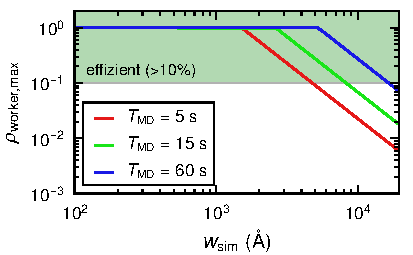
\includegraphics[width=\textwidth]{densitybymdtime}
  \end{subfigure}
  \hfill
  \begin{subfigure}[t]{\subfigwidth}
    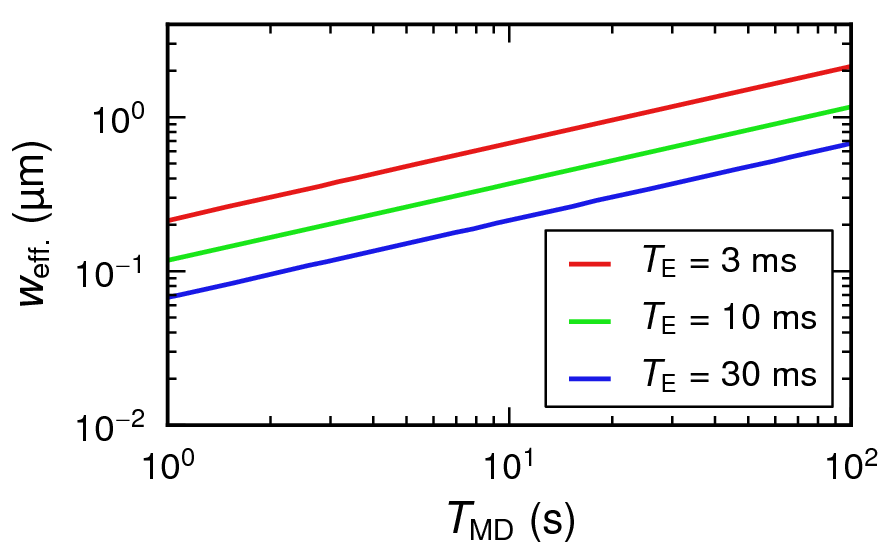
\includegraphics[width=\textwidth]{maxsizebymdtime}
  \end{subfigure}

  \caption{Einfluss der MD-Laufzeit auf die maximale Workerdichte und das Maximum der Simulationsgröße für effiziente Rechnungen ($\rho_\text{worker} > \SI{10}{\percent}$)}
  
\end{figure}

\begin{figure}
  
  \captionsetup[subfigure]{singlelinecheck=false}
  \def\subfigwidth{7cm}
  \begin{subfigure}[t]{\subfigwidth}
    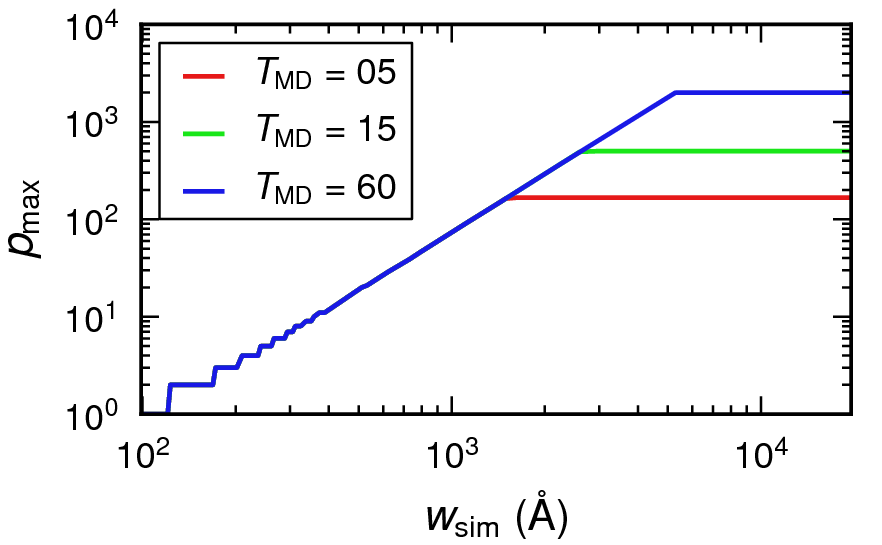
\includegraphics[width=\textwidth]{workersbymdtime}
  \end{subfigure}
  \hfill
  \begin{subfigure}[t]{\subfigwidth}
    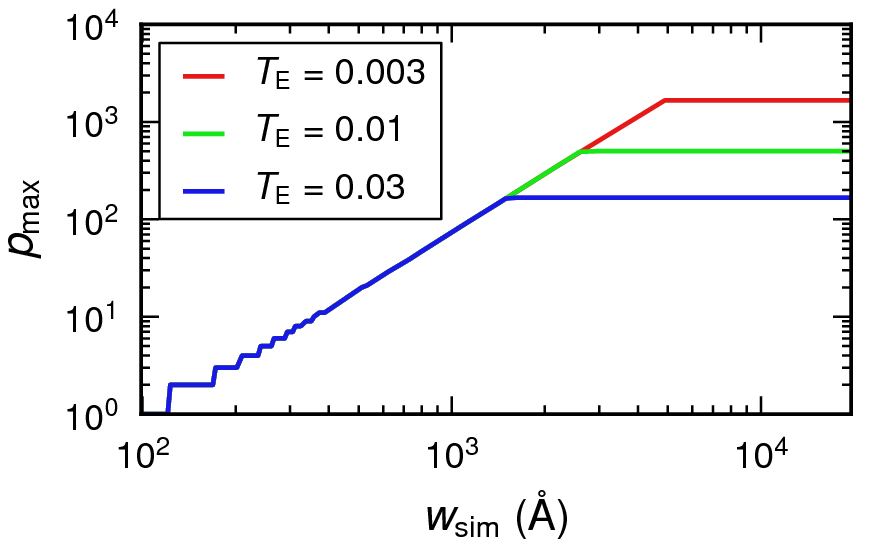
\includegraphics[width=\textwidth]{workersbykmctime}
  \end{subfigure}

  \caption{Einfluss der Ereignis-Laufzeit $T_\text{E}$ und der MD-Laufzeit $T_\text{MD}$ auf die maximale Zahl paralleler Prozesse $p_\text{max}$}
  
\end{figure}

\begin{figure}
  
  \captionsetup[subfigure]{singlelinecheck=false}
  \def\subfigwidth{7cm}
  \begin{subfigure}[t]{\subfigwidth}
    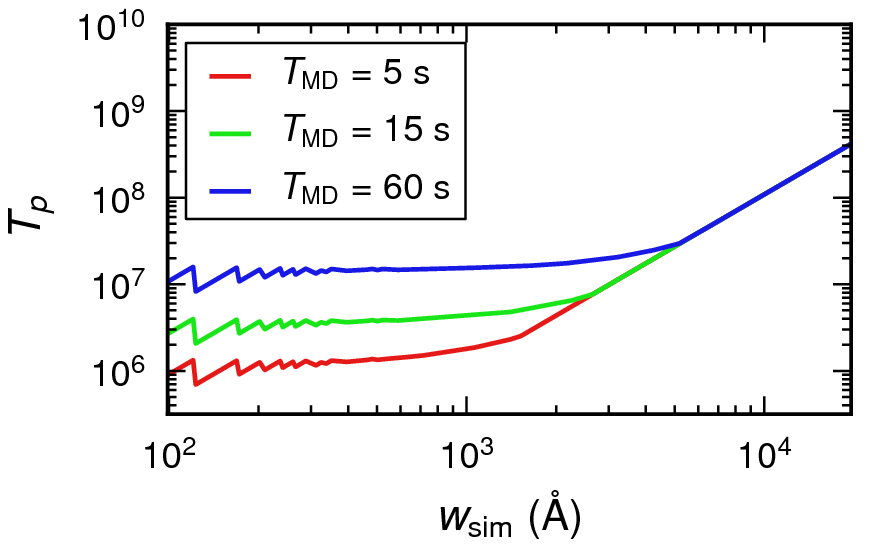
\includegraphics[width=\textwidth]{runtimebymdtime}
  \end{subfigure}
  \hfill
  \begin{subfigure}[t]{\subfigwidth}
    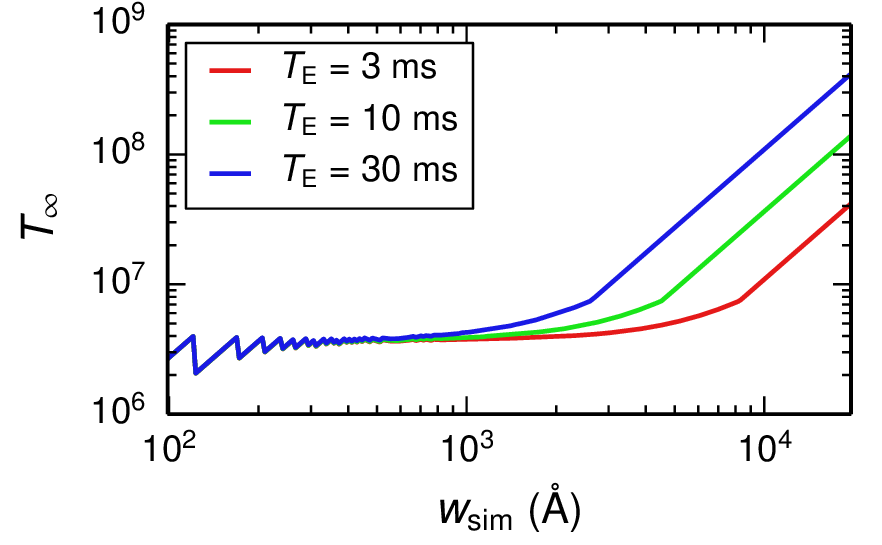
\includegraphics[width=\textwidth]{runtimebykmctime}
  \end{subfigure}

  \caption{Einfluss der Ereignis-Laufzeit $T_\text{E}$ und der MD-Laufzeit $T_\text{MD}$ auf die minimale Laufzeit $T_{p_\text{max}}$ einer Parsivald-Simulation}
  
\end{figure}

\todoline[Fazit]

, bei der sich die Ereignis-Laufzeit $T_\text{E}$, die MD-Laufzeit $T_\text{MD}$ und die Breite des Simulationsraumes $w_\text{sim}$ als ausschlaggebende Faktoren heraus stellen.
